
\section*{Problem 3}
Consider the network shown in Figure 2 and assume that each node initially knows the cost to each of its neighbors.
Consider the distance vector algorithm and consider the synchronous version that we discussed in class.
Answer the following questions

\begin{enumerate}
      \item Give the initial distance table of all the nodes.
      \item In the first round of exchange of distance vectors many distance vectors will node Z receive?
      \item Determine the distance table of node Z after the first round of exchange of distance vectors among
            the nodes.
\end{enumerate}

\begin{figure}[H]
      \centering
      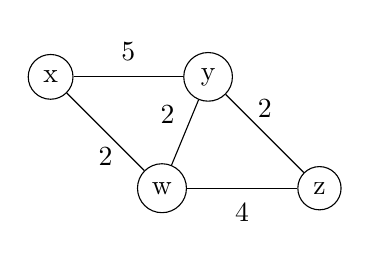
\begin{tikzpicture}
            \tikzstyle{every node} = [align=center, draw, circle, node distance = 2cm]
            \node(x){x};
            \node[right of=x](y){y};
            \node[below right of=x](w){w};
            \node[right of=w](z){z};

            \path (x) edge node[draw=none, below](){2} (w);
            \path (x) edge node[draw=none, above](){5} (y);
            \path (w) edge node[draw=none, above left](){2} (y);
            \path (w) edge node[draw=none, below](){4} (z);
            \path (y) edge node[draw=none, above](){2} (z);
      \end{tikzpicture}
      \caption{A four node network}
\end{figure}

\subsection*{Solution}

\begin{enumerate}
      \item The initial table is shown below:
            \begin{table}[H]
                  \centering
                  \begin{tabular}{lllll}
                        From $x$ & Via $x$ & Via $y$  & Via $z$ & Via $w$  \\
                        To $x$   & -       & -        & -       & -        \\
                        To $y$   & -       & 5        & NA      & $\infty$ \\
                        To $z$   & -       & $\infty$ & NA      & $\infty$ \\
                        To $w$   & -       & $\infty$ & NA      & 2
                  \end{tabular}

                  \vspace{5mm}

                  \begin{tabular}{lllll}
                        From $y$ & Via $x$  & Via $y$ & Via $z$  & Via $w$  \\
                        To $x$   & 5        & -       & $\infty$ & $\infty$ \\
                        To $y$   & -        & -       & -        & -        \\
                        To $z$   & $\infty$ & -       & 2        & $\infty$ \\
                        To $w$   & $\infty$ & -       & $\infty$ & 2
                  \end{tabular}

                  \vspace{5mm}

                  \begin{tabular}{lllll}
                        From $z$ & Via $x$ & Via $y$  & Via $z$ & Via $w$  \\
                        To $x$   & NA      & $\infty$ & -       & $\infty$ \\
                        To $y$   & NA      & 2        & -       & $\infty$ \\
                        To $z$   & -       & -        & -       & -        \\
                        To $w$   & NA      & $\infty$ & -       & 4
                  \end{tabular}

                  \vspace{5mm}

                  \begin{tabular}{lllll}
                        From $w$ & Via $x$  & Via $y$  & Via $z$  & Via $w$ \\
                        To $x$   & 2        & $\infty$ & $\infty$ & -       \\
                        To $y$   & $\infty$ & 2        & $\infty$ & -       \\
                        To $z$   & $\infty$ & $\infty$ & 4        & -       \\
                        To $w$   & -        & -        & -        & -
                  \end{tabular}


                  \caption{
                        ``-'': Connect to self, not applicable cell.
                        ``NA'': not directly connected, i.e. not neighbors.
                        ``$\infty$'': infinity length, as the actual min length is not known yet.
                  }
            \end{table}

      \item Two. Since at the first round $x$ has no idea how to connect to $z$.
      \item The table of $z$ after the first round is:
            \begin{table}
                  \centering
                  \begin{tabular}{lllll}
                        From $z$ & Via $x$ & Via $y$ & Via $z$ & Via $w$ \\
                        To $x$   & NA      & 7       & -       & 6       \\
                        To $y$   & NA      & 2       & -       & 6       \\
                        To $z$   & -       & -       & -       & -       \\
                        To $w$   & NA      & 4       & -       & 4
                  \end{tabular}
                  \caption{
                        ``-'': Connect to self, not applicable cell.
                        ``NA'': not directly connected, i.e. not neighbors.
                        ``$\infty$'': infinity length, as the actual min length is not known yet.
                  }
            \end{table}

\end{enumerate}

